\documentclass[times, utf8, diplomski, numeric, english]{fer}

\usepackage{booktabs}
\usepackage{amsmath}
\usepackage{nccmath}
%\usepackage{hyperref}
\usepackage[section]{placeins}

\usepackage{footnote}
\usepackage{graphicx}
\usepackage{float}
\usepackage{mathtools}
\usepackage{makecell}
\usepackage[hidelinks]{hyperref}

\renewcommand\theadalign{cb}
\renewcommand\theadfont{\bfseries}
\renewcommand\theadgape{\Gape[4pt]}
\renewcommand\cellgape{\Gape[4pt]}

\DeclarePairedDelimiter\ceil{\lceil}{\rceil}
\DeclarePairedDelimiter\floor{\lfloor}{\rfloor}

\DeclareMathOperator*{\argmin}{\arg\!\min}
\DeclareMathOperator*{\argmax}{\arg\!\max}
\begin{document}


\thesisnumber{1417}
\title{Deep Learning Model for Base Calling of MinION Nanopore Reads}
\author{Marko Ratković}

\maketitle

% Ispis stranice s napomenom o umetanju izvornika rada. Uklonite naredbu \izvornik ako želite izbaciti tu stranicu.
\izvornik

% Dodavanje zahvale ili prazne stranice. Ako ne želite dodati zahvalu, naredbu ostavite radi prazne stranice.
\zahvala{I would like to thank my mentor, Mile Šikić, for his patient guidance, encouragement
	and advice provided over the years.
	
I would also like to thank my family and friends for their
	continuous support.
	
In the end, honorable mentions go to Neven Miculinić for his help with this thesis.
	
}

\tableofcontents
\listoffigures
\listoftables

%%%%%%%%%%%%%%%%%%%%%%%%%%%%%%%%%%%%%%%%%%%%%%%%%%%%%%%%%%%%%%%%%%%%%%%%%%%%%%%%%%%%%%%
%% CHAPTER
\chapter{Introduction}

In recent years,  deep learning methods significantly improved the state-of-the-art in multiple domains such as computer vision, speech recognition, and natural language processing \cite{LeCun:1998:CNI:303568.303704}\cite{NIPS2012_4824}. 
In this thesis, we present application of deep learning in the field of  Bioinformatics for analysis of DNA sequencing data. 

DNA is a molecule that makes up the genetic material of a cell, and it is responsible for carrying the information needed for survival, growth, and reproduction of an organism. 
DNA is a long polymer of simple blocks called nucleotides connected together forming two spiraling strands to a structure called a double helix.  Possible nucleotide bases of a DNA strand are adenine, cytosine, guanine, thymine usually represented with letters A, C, G, and T. The order of these bases is what defines genetic code.

DNA sequencing is the process of determining this sequence of nucleotides. Originally sequencing was an expensive process, but during the last couple of decades, the price of sequencing has drastically decreased.  A significant breakthrough occurred in May 2015 with the release of MinION sequencer by Oxford Nanopore making DNA sequencing inexpensive and more available, even for small research teams. 

Base calling is a process assigning sequence of nucleotides (letters) to the raw data generated by the sequencing device. Simply put, it is a process of decoding the output from the sequencer.


\section{Objectives}
The goal of this thesis is to show that the accuracy of sequencing data is not only limited by sequencing technology, but also by the underlying software used for base calling and can be further improved using different machine learning concepts. A novel approach for base calling of raw data using convolutional neural networks is introduced.

\section{Organization}
\indent Chapter 2 gives more detailed explanation of the problem, background on nanopore sequencing and overview of state-of-the-art basecallers.

Chapter 3 describes in detail deep learning concepts used in later chapters.

Chapter 4 goes into implementation details, preprocessing methods and training of the deep learning model. 

Chapter 5 explains the methodology used to evaluate obtained results and the results of testing performed on different datasets as well as comparison with state-of-the-art basecallers.

In the end, Chapter 6 gives a brief conclusion and possible future work and improvements of the developed basecaller.

%%%%%%%%%%%%%%%%%%%%%%%%%%%%%%%%%%%%%%%%%%%%%%%%%%%%%%%%%%%%%%%%%%%%%%%%%%%%%%%%%%%%%%%
%% CHAPTER
\chapter{Background}

\section{Sequencing}

All sequencing technologies to date have constraints on the length of the strand they can process, which are much smaller than the genome for a majority of organisms, making sequencing the entire genome of an organism a difficult problem. To resolve this problem whole genome shotgun sequencing approach is used, in which multiple copies of the genome are broken randomly into numerous small fragments that can be processed by the sequencer. Sequenced fragments are called reads.

Genome assembly is the process of reconstructing the original genome from reads and usually starts with finding overlaps between reads.
The quality of reconstruction heavily depends on the length and the quality (accuracy) of the reads produced by the sequencer.

Figure \ref{fg:sequencing} depicts process of sequencing.

\begin{figure}[!ht]
	\begin{center}
		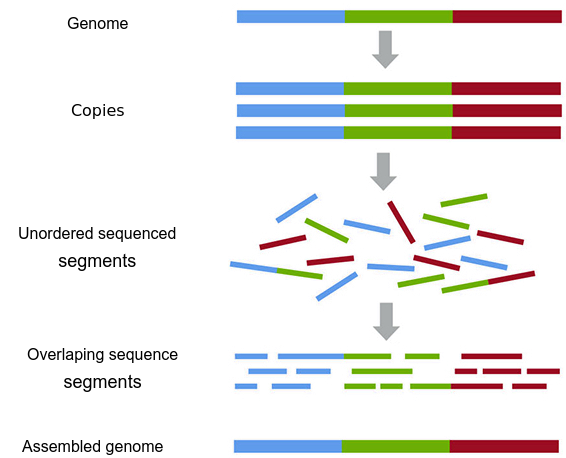
\includegraphics[width=0.6\textwidth]{./imgs/sequencing.png}
		\caption{Depiction of the sequencing process}
		\label{fg:sequencing}
	\end{center}
\end{figure}


Development of sequencing started with work of Frederick Sanger \cite{mile} \cite{Pettersson2009}. In 1977, he developed the first sequencing method which allowed 
read lengths up to 1000 bases with very high accuracy (99.9\%) at the cost of 1\$ per 1000 bases.
Second generation sequencing (IAN Torrent and Illumina devices) reduced the price of sequencing while maintaining high accuracy. Mayor disadvantage of these devices is read length of only a few hundred base pairs. Short reads make resolving repetitive regions practically impossible.

The need for technology able of producing longer reads led to the development of so-called third generation sequencing technologies.
PacBio developed sequencing method that allowed read lengths up to several thousand bases but at the cost of smaller accuracy. Error Rates of PacBio devices are \textasciitilde10-15\%. 

Cost makes the biggest obstacle stopping widespread genome sequencing. The release of, previously mentioned, MinION sequencer made sequencing less expensive and even portable.



\section{Oxford Nanopore MinION}

The MinION device by Oxford Nanopore Technologies is the first portable DNA sequencing device. Its small weight, low cost, and long read length combined with decent accuracy yield promising results in various applications including full human genome assembly \cite{human_seq} what could potentially lead to personalized genomic medicine.

\subsection{Technology}
As its name says, nanoscaled pores are used to sequence DNA. An electrical potential is applied over a membrane in which a  pore is inserted. 
As the DNA passes through the pore, the sensor detects changes in ionic current caused by different nucleotides present in the pore. Figure \ref{fg:nanopore} shows the change of ionic current as DNA strain is pulled through a nanopore.

\begin{figure}[!ht]
	\begin{center}
		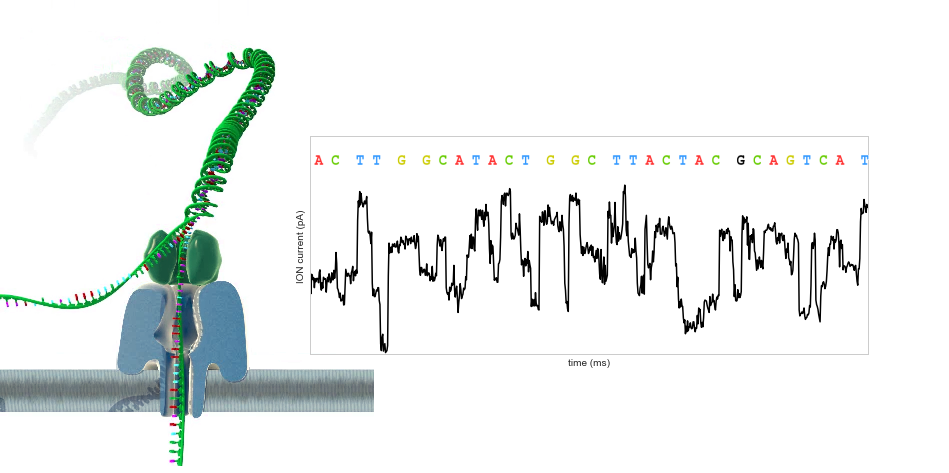
\includegraphics[width=0.7\textwidth]{./imgs/nanopore.png}
		
		\caption[DNA strain being pulled through a nanopore]{DNA strain being pulled through a nanopore \protect\footnotemark}
		\label{fg:nanopore}
	\end{center}
\end{figure}
\footnotetext{Figure adapted from https://nanoporetech.com/how-it-works}


Official software called MinKNOW outputs sequencing data in FAST5 (a variant of the HDF5 standard) file format. It is a hierarchical file format with data arranged in a tree-structure of groups. Metadata are stored in group and dataset attributes. The same file format is during used different stages of analyses and groups, datasets and attributes are added incrementally. Figure \ref{fg:fast5} shows raw signal being present in the FAST5 file.
\begin{figure}[!ht]
	\begin{center}
		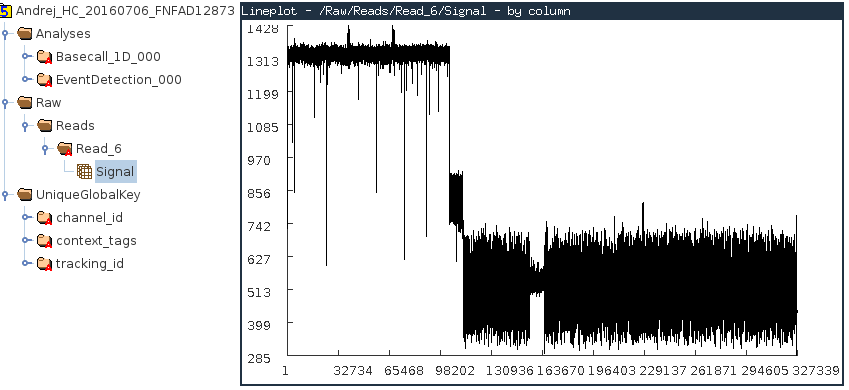
\includegraphics[width=0.6\textwidth]{./imgs/fast5.png}
		\caption[Structure of FAST5 file and raw signal plot show in \textit{HDFView}]{Structure of FAST5 file and raw signal line plot show in \textit{HDFView} \protect\footnotemark}
		\label{fg:fast5}
	\end{center}
\end{figure}
\footnotetext{https://support.hdfgroup.org/products/java/hdfview/}

Minion offers the possibility of sequencing one or both strands of DNA. Sequencing both strands and combining information results in reads of higher quality. Those reads are called 2D (two-dimensional) reads. Otherwise, if the only single strand is sequenced 1D (one-dimensional) reads are produced.

MinION devices can produce long reads, usually tens of thousand base pairs (with reported reads lengths of 100 thousand \cite{loman1-100k} and even recently above 800 thousand base pairs \cite{loman2-800k}), but with high sequencing error than older generations of sequencing technologies.
Switch from older R7.3 to  R9 chemistry in 2016 increased accuracy of produced data. With this change, the accuracy of 1D data increased from 70\% to 85\% and the accuracy of 2D reads from 88\% to 94\% \cite{nanopore_video}.  This increase of accuracy makes 1D reads usable for analysis with benefits over 2D reads being faster sample preparation and faster sequencing. Developed tool in this thesis focuses on base calling 1D reads.


  
\section{Existing basecallers}

\subsection{Official}
Oxford Nanopore has, with the R9 version of the platform, introduced a variety of base calling options. Some of those are production ready and some experimental. The majority of information regarding differences, specifications and similar is only available through Nanoporetech Community \footnote{https://community.nanoporetech.com/}.


\textit{Metrichor} is an Oxford Nanopore company that offers cloud-based platform \textit{EPI2ME} for analysis of nanopore data. 
Initially, base calling was only available by uploading data to the platform - that being the reason why this basecaller is often called Metrichor even though it is a name of the company.

The older version of Metrichor relied on \textit{hidden Markov models} (HMM) to find the biological sequence corresponding to the signal. Preprocess included segmentation of the signal into smaller chunks called events defined by start location of the chunk, length, mean value and variance of the signal in the chunk. Metrichor than assumed that each event usually corresponds to a context of 6 bases being present in the pore and that the context is typically shifted by one base in each step. 
The states of HMM are modeled as a context present in the pore and transition correspond to change of bases in the pore. During the transition from one state to another, an event is emitted. Base calling is performed using the Viterbi algorithm which determines the most likely sequence of states for the observed sequence of events. This approach showed poor results when calling long homopolymer stretches as the context in the pore remains the same \cite{homopolymers}\cite{homopolimeri_analiza}.

With the release of R9 chemistry, this model was replaced by a more accurate recurrent neural network (RNN) implementation. Currently, Oxford Nanopore offers several RNN-based local basecaller versions under different names: Albacore, Nanonet and basecaller integrated into MinKNOW \cite{ont-basecallers}.   

\textit{Albacore} is basecaller by Oxford Nanopore Technologies ready for production and actively supported.
It is available to the Nanopore Community served as a binary. The source code of Albacore was not provided and is only available through the ONT Developer Channel. Tool supports only R9.4 and future R9.5 version of the chemistry.

\textit{Nanonet}\footnote{\url{https://github.com/nanoporetech/nanonet/}} uses the same neural network that is used in Albacore but it is continually under development and does contain features such as error handling or logging needed for production use. It uses \textit{CURRENNT} library for running neural networks. It supportes basecalling of both R9 and R9.4 chemistry versions.


\textit{Scrappie}\footnote{\url{https://github.com/nanoporetech/scrappie}} is another basecaller by Oxford Nanopore Technologies. Similar to Nanonet, it is the platform for ongoing development. Scrappie is reported to be the first basecaller  that specifically address homopolymer base calling. It became publicly available just recently in June, 2017 and supports R9.4 and future R9.5 data.

\pagebreak
\subsection{Third-party basecallers}

\textit{Nanocall} \cite{David046086} was the first third-party open source basecaller for nanopore data. It uses HMM approach like the original R7 Metrichor. Nanocall does not support newer chemistries after R7.3.


\textit{DeepNano} \cite{Boza2017}  was the first open-source basecaller based on neural networks. It uses bidirectional recurrent neural networks implemented in Python, using the Theano library. When released, originally only supported R7 chemistry, but support for R9 and R9.4 was added recently.



%%%%%%%%%%%%%%%%%%%%%%%%%%%%%%%%%%%%%%%%%%%%%%%%%%%%%%%%%%%%%%%%%%%%%%%%%%%%%%%%%%%%%%%
%% CHAPTER
\chapter{Methods}
The process of base calling can be represented as the problem of machine translation where a sentence is translated from one language to another. For base calling, the sequence of events or current measurements is \textit{translated} to the sequence of nucleotides (letters A, C, T, and G).

This section explains some key  deep learning concepts needed to understand the final model. It gives general idea behind recurrent neural networks used in a majority of existing basecallers and possible problems that serve as motivation for the different approach - usage of convolutional neural networks. 

\section{Architecture}

\subsection{RNN}
\textit{Recurrent neural networks} can be viewed as a simple feed-forward network with the difference that the current output does not only depend on the current input but previous inputs as well. RNNs store that information in their hidden state which is updated in each step. The figure shows simple RNN and the same RNN unfolded in time.  Unrolling is a way of showing how network processes each input in the sequence and updates its hidden state (show in figure  \ref{fg:rnn}).
\begin{figure}[!ht]
	\begin{center}
		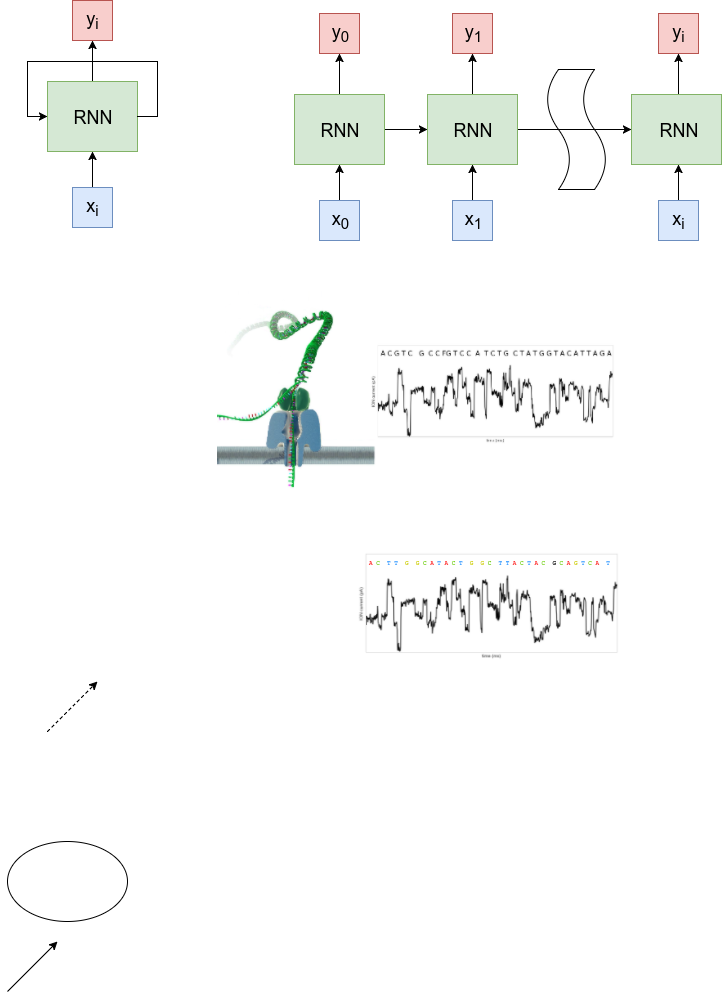
\includegraphics[width=0.8\textwidth]{./imgs/rnn.png}
		\caption{An unrolled recurrent neural network}
		\label{fg:rnn}
	\end{center}
\end{figure}

These networks are trained using a variant of backpropagation called backpropagation through time which is essentially the same as classical backpropagation on an unfolded network. The gradient is propagated through the entire recurrence relation, and the gradient is multiplied in each step with the factor, depending on a scale it can make gradient vanish (drop to 0) or exponentially grow each step and explode. Detailed explanation can be found \cite{rnn-blog}. These issues are called the vanishing and exploding gradient and are generally resolved by a variant of RNN called \textit{LSTM} \cite{hochreiter1997long}. 

Bidirectional Recurrent Neural (BiRNN) networks are used when the current output not only depends on the previous elements in the sequence but also future elements. The idea is to combine two RNN (one in the positive direction, one in negative time direction) and have an output of the current state expressed as a function of hidden states of both RNNs and current input. This is the approach used in DeepNano \cite{Boza2017}. 


One of the major drawbacks of all recurrent networks is computation time. RNNs operate sequentially as the output for the second step depends on the first step and so on, which makes parallelization capabilities of RNNs quite limited. This especially is the case for Bidirectional RNNs.

\subsection{CNN}

\textit{Convolutional Neural Networks }(CNNs) were responsible for major breakthroughs in Image Classification and are the core of most Computer Vision systems today. More recently CNNs are applied being to problems in Natural Language Processing and show promising results \cite{BYTENET}\cite{facebook}.

Convolution can be easily explained as a sliding window function applied to a matrix or in the case of base calling, signal. The sliding window is called a kernel or a filter. Figure \ref{fg:convolution} shows an example of convolution with kernel size 3 and how output is calculated as a sum of element-wise multiplication of kernel elements and input vector. Stride defines by how much filter is shifted at each step. Usually, to preserve the same dimension, padding with zeros is added to the borders. 

\begin{figure}[H]
	\begin{center}
		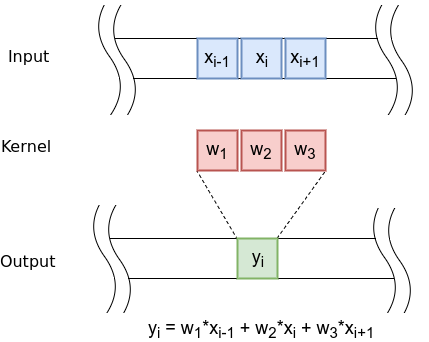
\includegraphics[width=0.5\textwidth]{./imgs/convolution.png}
		\caption{Convolution layer, kernel size 3 with stride 1.}
		\label{fg:convolution}
	\end{center}
\end{figure}


\subsubsection{Activations}
After each convolution layer, usually nonlinear layer (know as activation layer) is applied. The purpose of this layer is to introduce nonlinearity to a system which consists of only linear operations as convolution layers are nothing more than just element-wise multiplications and summations. In classical neural networks, nonlinear functions like $ tanh $ and $ sigmoid $ were often used, but because of the undesirable property of saturation (at either end of 0 or 1 for $ sigmoid $, -1 or 1 for $ tanh $), other activations are more often used today with CNNs. 

\textit{The Rectified Linear Unit }(ReLU) has become very popular in the last few years. It is shown in \cite{NIPS2012_4824} that usage of ReLU greatly accelerates the convergence of stochastic gradient descent compared to the sigmoid or tanh activations. Calculation of ReLU is much also more efficient as it is is simply thresholding at zero. 

\begin{equation}
ReLU(x) =
\begin{cases}
x, & \text{if}\ x>0 \\
0, & \text{otherwise}
\end{cases} \\
\end{equation}


The downside of ReLU is still saturation to the 0 on one side. Once in this state, the neuron is unlikely to recover because the function gradient at 0 is also 0, so gradient descent learning will not alter the weights. This is the problem known as \textit{dying ReLU}.
Different variants of ReLU, \textit{PrRelu}, and \textit{ELU} are often used to resolve this problem \cite{prelu}\cite{elu}.  

\begin{equation}    
PrELU(x)=
\begin{cases}
x, & \text{if}\ x>0 \\
\alpha x, & \text{otherwise}
\end{cases}\\
\end{equation}
\begin{equation}
ELU(x)=
\begin{cases}
x, & \text{if}\ x>0 \\
\alpha (exp(x) - 1), & \text{otherwise}
\end{cases}    \\
\end{equation}

Figure \ref{fg:activations} shows different activation functions.
\begin{figure}[!htb]
	\begin{center}
		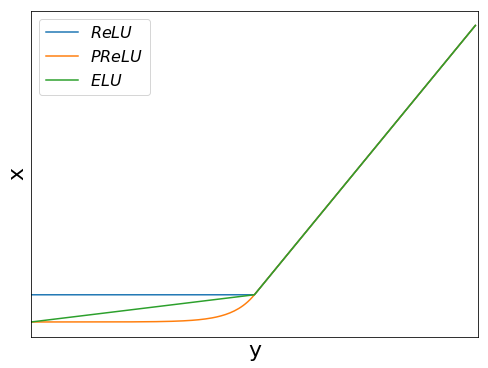
\includegraphics[width=0.5\textwidth]{./imgs/activations.png}
		\caption{Activation functions}
		\label{fg:activations}
	\end{center}
\end{figure}

\subsubsection{Pooling}

The pooling layer is usually placed after the convolutional layer. Its primary utility lies in reducing the spatial dimensions of the input for the next convolution layer while preserving the most salient information. Pooling also provides basic invariance to translation.

Similar to the convolution layer described previously, the pooling layer also uses sliding window or a certain size that is moved across the input transforming the values. Usually, larger strides are used then in the convolution layers, as the purpose of this layer is subsampling. Most ofter, maximum value operation on the values in the window (max pooling) is used, but other transformations are possible (average pooling, L2-norm, or stochastic pooling).
Figure \ref{fg:pooling} show dimensionality reduction by factor 2 using pooling with kernel size 2 with stride 2.
\begin{figure}[!htb]
	\begin{center}
		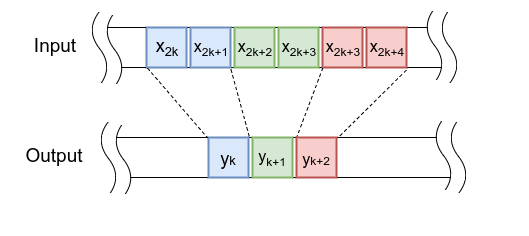
\includegraphics[width=0.5\textwidth]{./imgs/pooling.png}
		\caption{Dimensionality reduction by pooling (kernel size 2, stride 2)}
		\label{fg:pooling}
	\end{center}
\end{figure}




  
\subsubsection{Comparision with RNN}


During calculation, each \textit{patch} a convolutional kernel operates on is independent of the other, meaning that the entire input layer can be processed concurrently making CNNs usually more efficient than RNNs. 

When compared with RNN in which output can depend on the entire sequence,  in convolution layer, single output \textit{sees} only limited window in the previous layer defined by kernel size. This is called the receptive field of the convolution. 
Figure \ref{fg:receptive field} shows each new layers depends on larger portion of the input ($z_i$ \textit{sees} 5 elements of input). 
Lower layers see limited spatial information and are able to detect simple features like edges but through a series of convolutional layers, later layers can detect more abstract concepts using intermediate features detected from the whole input, or the signal in our case. This is the motivation behind deep convolution neural networks and why they are so popular in the field of image processing.

\begin{figure}[!ht]
	\begin{center}
		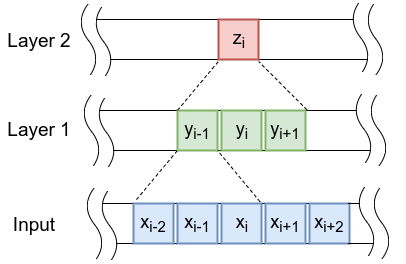
\includegraphics[width=0.5\textwidth]{./imgs/receptive_field.png}
		\caption{Receptive field after 2 layers of convolutions with kernel size 3}
		\label{fg:receptive field}
	\end{center}
\end{figure}
Stacking layers increases computational time as the input signal has to pass through the entire network but calculations at each layer can happen concurrently and each individual computation is small.
In practice, even deep CNNs still have a big speed up over RNNS.

During the forward pass, input flows and is transformed, hopefully becoming a representation that is more suitable for the task. During the back phase, the gradient is propagated back through the network. Just like in RNNs, this signal gets multiplied and depending on the scales it can vanish resulting in no gradient flow to lower layers and no parameter upgrades. This limits the depth of the network. Resnet arhitecture \cite{resnet} with its residual layers address this issue and allows deep architectures with steady gradient flow.




\subsection{Residual Networks}
A Residual Network or ResNet is a neural network architecture which solves the problem of vanishing gradients using a simple trick.  
Figure \ref{fg:resnet_block}  shows on the left classical CNN that takes input and transforms it using convolution layers and activations.  This can be represented as some nonlinear function $ H(x) $. $ H(x) $ can be written as a sum of some other nonlinear function $F(X)$ and linear member $x$. $F(X) $ is called the residual. Detailed explanation and comparisons are included in the original paper.

\begin{figure}[!ht]
	\begin{center}
		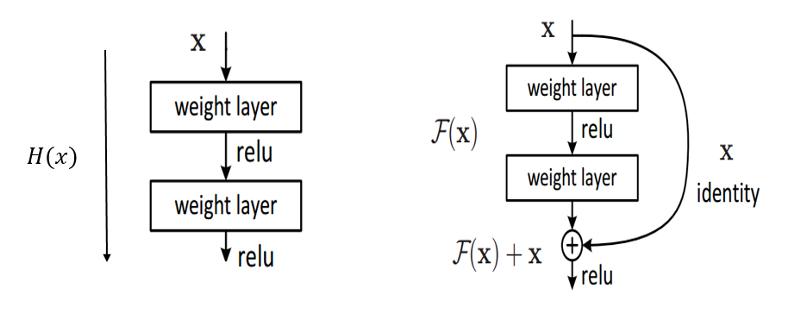
\includegraphics[width=0.7\textwidth]{./imgs/resnet_block.png}
		\caption[Comparison between classical CNN and CNN with the residual connection ]{Comparison between classical CNN and CNN with the residual connection \protect\footnotemark}
		\label{fg:resnet_block}
	\end{center}
\end{figure}
\footnotetext{Figure adapted from the original paper \cite{resnet}}
Instead of learning $H(X)$, network learns residual and at the output $x$ is simply summed up to the $F(x)$ as shown in the figure.  By stacking these layers, the gradient could theoretically \textit{skip} over all the intermediate nonlinear layers and reach the bottom without vanishing.




\section{CTC Loss}

As mentioned previously, the goal of this thesis is to design model which can convert from a sequence of current measurements into a sequence of base pairs.

Suppose that we have an input sequence $X$ (signal data) and the desired output sequence $Y$ (nucleotides). $X$ and $Y$ will be of different lengths as the sequence of base pairs is always shorter than the length of the signal.

Instead of having a variable size of the output from the neural network, we can limit it to the length $m$ and have sequences of variable length \textit{decoded} from those outputs. The neural network can be considered to be simply a function that takes in some input sequence $X$ (of length $n$) and generates sequence $O$ (of length $m$). Output sequence of variable length $Y$ is later \textit{decoded} from $O$.

\subsection{Definition}
They key idea behind Connectionist Temporal Classification(CTC) \cite{Graves:2006:CTC:1143844.1143891} is that instead of directly generating output sequence $Y$ as output from the neural network, we  generate a probability distribution at every output length (from $t$=1 to $t$=$m$) that after \textit{decoding} gives maximum likelihood output sequence $Y$. 
Finally, the network is trained using training dataset $D = \{(X_i, Y_i)\}$ by creating an objective function that restricts the maximum likelihood decoding for a given sequence $X_i$ to correspond to our desired target sequence $Y_i$.

Given an input sequence $X$ of length $n$, the network generates probabilities over all possible labels (A, C, T, and G) with an extra symbol "-" representing a \textit{blank} at each timestep. 
\begin{equation}
\begin{gathered}
\Sigma = \{A, C, T, G\} \cup \{-\}
\end{gathered}
\end{equation}


Possible output generated by the network is called \textit{path}. Path is defined by the sequence of its elements $\pi = (\pi_1, \pi_2, ..., \pi_m)$ where $\pi_i$ is from $\Sigma$.
The probability of a given path $\pi$, given input sequence $X$, can then be expressed as the product of probabilities for each of its forming elements.

\begin{equation}
\begin{gathered}
P(\pi | X) = \prod_{t=1}^{m} o_t(\pi_t), \\
\text{where $o_t(\pi_t)$ is probability of element $\pi_t$ being $t^{th}$ element on path $\pi$}
\end{gathered}
\end{equation}


Real output sequence, for given path, is obtained by traversing the path and removing all blanks and duplicate letters. Let $ decode(\pi) $ be the output sequence corresponding to a path $\pi$. As seen
in expression \ref{eq:multiple} multiple path correspond to the same sequence $Y="ACT"$.
\begin{equation}
\begin{gathered}
\label{eq:multiple}
ACT = \begin{cases}
decode(A, A, A, C, T) \\
decode(A, A, C, -, T) \\
decode(-, A, C, T, T)  \\
decode(-, -, A, C, T)  \\
decode(A, C, C, C, T)  \\
\vdots \\
decode(A, C, T, -, -) 
\end{cases}
\end{gathered}
\end{equation}

The probability of output sequence $Y$ is then the sum of probabilities of all paths that decode to $Y$:
\begin{equation}
\begin{gathered}
P(Y | X) = \sum_{\pi \in decode^{-1}(Y)}^{} P(\pi | X)
\end{gathered}
\end{equation}
\subsection{Objective}
Given the dataset $D = \{(X_i, Y_i)\}$, training objective is the maximization of the likelihood of each training sample  which is the same as the minimization of negative log likelihood:

\begin{equation}
\begin{gathered}
L(D) = - \sum_{(X,Y)\in D}^{} ln P(Y | X)
\end{gathered}
\end{equation}


\subsection{Output decoding}
Given the probability distribution $P(Y | X)$ and given input sequence $X$, most likely $Y^{*}$ can be computed.
\begin{equation}
\begin{gathered}
Y^{*} = \argmax_{Y \in L^m} P(Y|X) = \argmax_{Y \in L^m} \sum_{\pi \in decode^{-1}(Y)}^{} P(\pi | X),\\
\text{~where $L^m$ set of all possible sequences over alphabet $L$ }\\
\text{with length less than or equals to $m$}
\end{gathered}
\end{equation}

The probability of a single output sequence $Y$ is the sum of probabilities of all paths that decode to $Y$ and the most probable sequence is selected as the output.
Calculation of all possible sequences is computationally intractable but exist several algorithms that approximate this decoding. 

The naive possibility is to take the most probable path and say that output sequence corresponds to that path.
This is not necessarily correct.  For example, suppose we have one path with probability $0.1$ corresponding to sequence $A$, and ten paths with probabilities  $0.05$ each corresponding to sequence $B$. Label $B$ is preferable one since it has an overall probability of $0.5$; however, this naive best path decoding would select label $A$, whose single path has higher probability the those for label $B$. This method is called \textit{best path decoding}.

Better approximations can be calculated using \textit{beam search decoding} proposed in paper \cite{graves_decode}.  
The idea is an incremental construction of the most probable sequences in step $t$ using $N$ most probable sequences from the previous step. Parameter $N$ is called beam width. 




Probability of $Y$ being extended with character $c$ in step $t$ is expressed like:
\begin{equation}
\begin{gathered}
P(c, Y, t) = P(Y, t-1) * p(c, t|X), \\\text{~where $p(c, t|X)$ is probability of $c$ being t-th output from the network in t-th step}.
\end{gathered}
\end{equation}

Lets label  with $\hat{Y}$ prefix of $Y$ without last symbol and $Y^e$ as last symbol in $Y$.
\begin{equation}
\begin{gathered}
Y = \hat{Y} + Y^e, \text{~where $+$ is concatanation operator}
\end{gathered}
\end{equation}


We can get $Y$ by having $\hat{Y}$ in previous step and network output $Y^e$ or simply by
already having $Y$ in previous step and network output blank($-$) or $Y^e$ as blanks and repeats are merged during decoding.
\begin{equation}
\begin{gathered}
\label{eq:rec_step}
P(Y, t) = P(Y, t-1) p(-, t|X) +  P(Y, t-1)  p(Y^e, t|X) +  P(\hat{Y}, t-1)  p(Y^e, Y, t) 
\end{gathered}
\end{equation}
Using this expression, using dynamic programing can efficiently be determine probability of some sequence $Y$.

Beam search decoder keeps set $B$ of $N$ most probable sequences. $B$ is initially a set consisting of a single blank. In each time step $t$ (from $t$=1 to $t$=$m$) all sequences from $B$ are expanded and probabilities of new sequences are calculated using recursive relation \ref{eq:rec_step}. Expanded sequences are placed in the new set $B'$. At the end of each step, $B$ is replaced by $B'$ and truncated by keeping $N$ most probable sequences. 
After last time step, the sequence in $B$ with the highest probability is chosen as the final output.
Full pseudocode can be found in original paper \cite{graves_decode}. 
Detailed explanation and calculation of gradient can be found in original CTC paper \cite{Graves:2006:CTC:1143844.1143891}, or this very detailed blog post \cite{ctc-blog}.


\section{Batch normalization}
Batch normalization is method proposed in paper \cite{BNORM} that accelerates learning process. 
During training, parameters are updated, and distribution of outputs of each layer keep changing. A small change in the distribution of outputs in early layers can cause a drastic change in later layers, and those layers need to adapt to the new scale of their inputs. This change of distribution is called the internal covariate shift and results in slows learning.
This is solved by centering each output from activations of the training batch to zero-mean and unit variance. After that learned scale and offset are applied. This process is called batch normalization. 
After training, mean and variance for each activation are computed on the whole training dataset rather than on mini-batches during training. 

Batch normalization offers several advantages other than reducing internal covariant shift including more robust learning process by reducing reliance on the scale of the parameters and their initial values allowing the usage of larger learning rates and faster learning altogether. It is shown in the original paper that batch normalization also regularizes the model that could potentially improve the performance of the model.

%%%%%%%%%%%%%%%%%%%%%%%%%%%%%%%%%%%%%%%%%%%%%%%%%%%%%%%%%%%%%%%%%%%%%%%%%%%%%%%%%%%%%%%
%% CHAPTER
\chapter{Implementation}


\section{Data}

Both used datasets show in table \ref{tbl:datasets} be previously have passed through MinKNOW and had been basecalled by Metrichor. As 1D read analysis was the focus of this thesis, only those reads were used.
\begin{savenotes}
	\begin{table}[htb]
		\caption{Used datasets}
		\label{tbl:datasets}
		\centering
		
		\begin{tabular}{lcc| c}
			\toprule
			{} &  \thead{Number of reads} &   \thead{Total bases \lbrack bp\rbrack\footnote{Total number of bases calle by Metrichor}} &    \thead{Whole genome size \lbrack bp\rbrack} \\
			\midrule
			\textit{{E. Coli}}\footnote{R9 sequencing data from \url{http://lab.loman.net/2016/07/30/nanopore-r9-data-release/}, reference taken from \url{https://www.ncbi.nlm.nih.gov/nuccore/48994873}} & 164471 & 1 481 687 490 & 4 639 675\\
			\textit{lambda}\footnote{Internal dataset, reference taken from \url{https://www.ncbi.nlm.nih.gov/nuccore/NC_001416.1}}   & 86 &  466 465 & 48 502  \\
			
			\bottomrule
		\end{tabular}
	\end{table}
\end{savenotes}


Figure \ref{fg:events} shows data present inside FAST5 file after being base calling by Metrichor. For each basecalled event, $model\_state$ field contains the most likely sequence of bases in the pore. How many bases have passed through the pore between two consecutive events is defined by the $move$ field. 


\begin{figure}[!ht]
	\begin{center}
		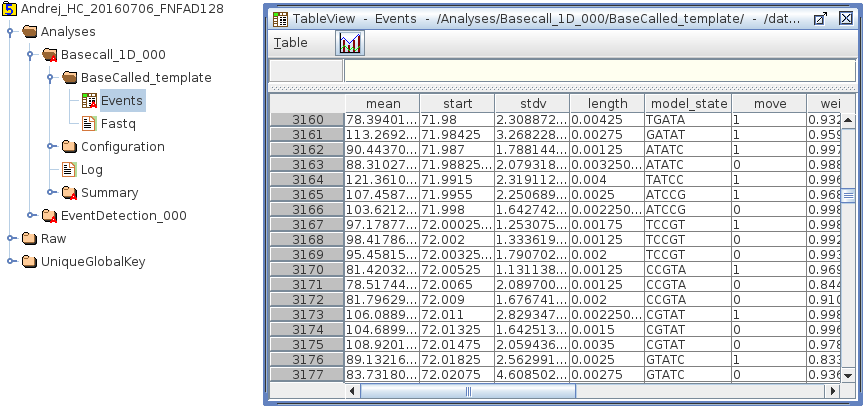
\includegraphics[width=1\textwidth]{./imgs/basecall_events.png}
		\caption{Basecall information produced by Metrichor show in HDFView}
		\label{fg:events}
	\end{center}
\end{figure}



\subsection{File formats}
Descriptions of various file formats used later in descriptions of preprocessing of training data and evaluation are given in this section.
\subsubsection{FASTA}


FASTA is widely used file format for reference sequences. Usual file extensions are \textit{.fasta} or \textit{.fa}).
Sequence representation consists of header line containing description starting with character $ > $, followed by line(s) of sequence data represented by letters. Full file specification can be found at \textit{NCBI} site\footnote{\url{http://www.ncbi.nlm.nih.gov/BLAST/blastcgihelp.shtml}}.
Figure \ref{fg:fsta} shows example of sequence stored in FASTA file format.
\begin{figure}[!ht]
	\begin{center}
		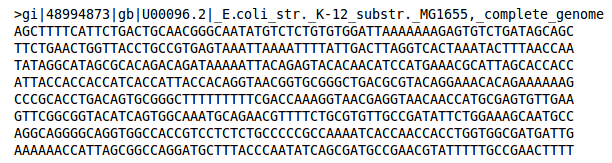
\includegraphics[width=0.8\textwidth]{./imgs/fasta.png}
		\caption{Example of FASTA file}
		\label{fg:fsta}
	\end{center}
\end{figure} 

\subsubsection{FASTQ format}
Reads are usually stored in FASTQ file format. Each read in the file is stored in following way:
\begin{enumerate}
	\item character "$@$" followed  by a sequence identifier and an optional description 
	\item sequence
	\item character "$+$" character and is optionally followed by the same sequence identifier and description.
	\item quality score for each base
\end{enumerate}
Quality is represented by ASCII printable characters where
the character "$!$" represents the lowest quality while "\textasciitilde" is the highest. Figure \ref{fg:fq} shows example of read stored in FASTQ file format.
\begin{figure}[!ht]
	\begin{center}
		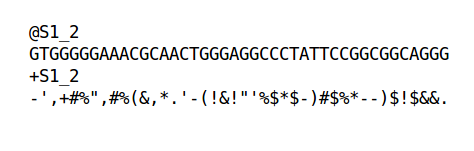
\includegraphics[width=0.6\textwidth]{./imgs/fq.png}
		\caption{Example of FASTQ file}
		\label{fg:fq}
	\end{center}
\end{figure} 

\subsubsection{SAM format}
The Sequence Alignment/Map (SAM) format is a generic format for storing reads alignments against the reference sequences. It is a TAB-delimited text format consisting
of header section and an alignments section. Detailed information about SAM specification can be found on \textit{SAMTools} website\footnote{\url{https://samtools.github.io/hts-specs/SAMv1.pdf}}.
Among other information, alignment start position is included, flag stating if read aligned as the template of as the reverse complement and CIGAR string describing the alignment.
Figure \ref{fg:align} shows simple alignment and CIGAR string. 
There are several possible letters that can appear in CIGAR string but most importantly matches, mismatches, insertions and deletions are represented by letters "=", "X", "I" and "D".


\begin{figure}[!ht]
	\begin{center}
		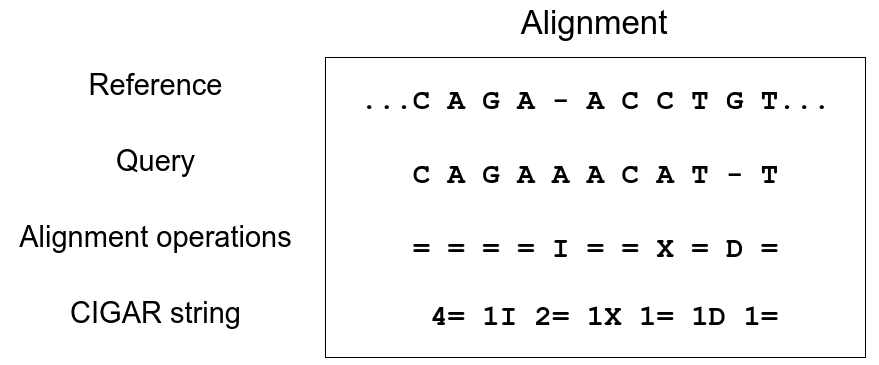
\includegraphics[width=0.6\textwidth]{./imgs/alignment.png}
		\caption{Example of simple alignment and CIGAR string}
		\label{fg:align}
	\end{center}
\end{figure} 


\section{Data preprocess}

To help training process, the raw signal is split into smaller blocks that are used as inputs. For each Metrichor basecalled event is easy to determine the block it falls into using $start$ field. Using this information output given by Metrichor can be determined for each block. 
To correct errors produced by Metrichor and possibly increase the quality of data, each read is aligned to the reference. This is done using aligner GraphMap \cite{sovic} that returns the best position in the genome, hopefully, the part of the genome from which read came from.
Alignment part in the genome is used as a target. Using CIGAR string returned by aligner we can correct Metrichor data and get target output for each block. This process is shown in figure \ref{fg:data_correction}.

\begin{figure}[!ht]
	\begin{center}
		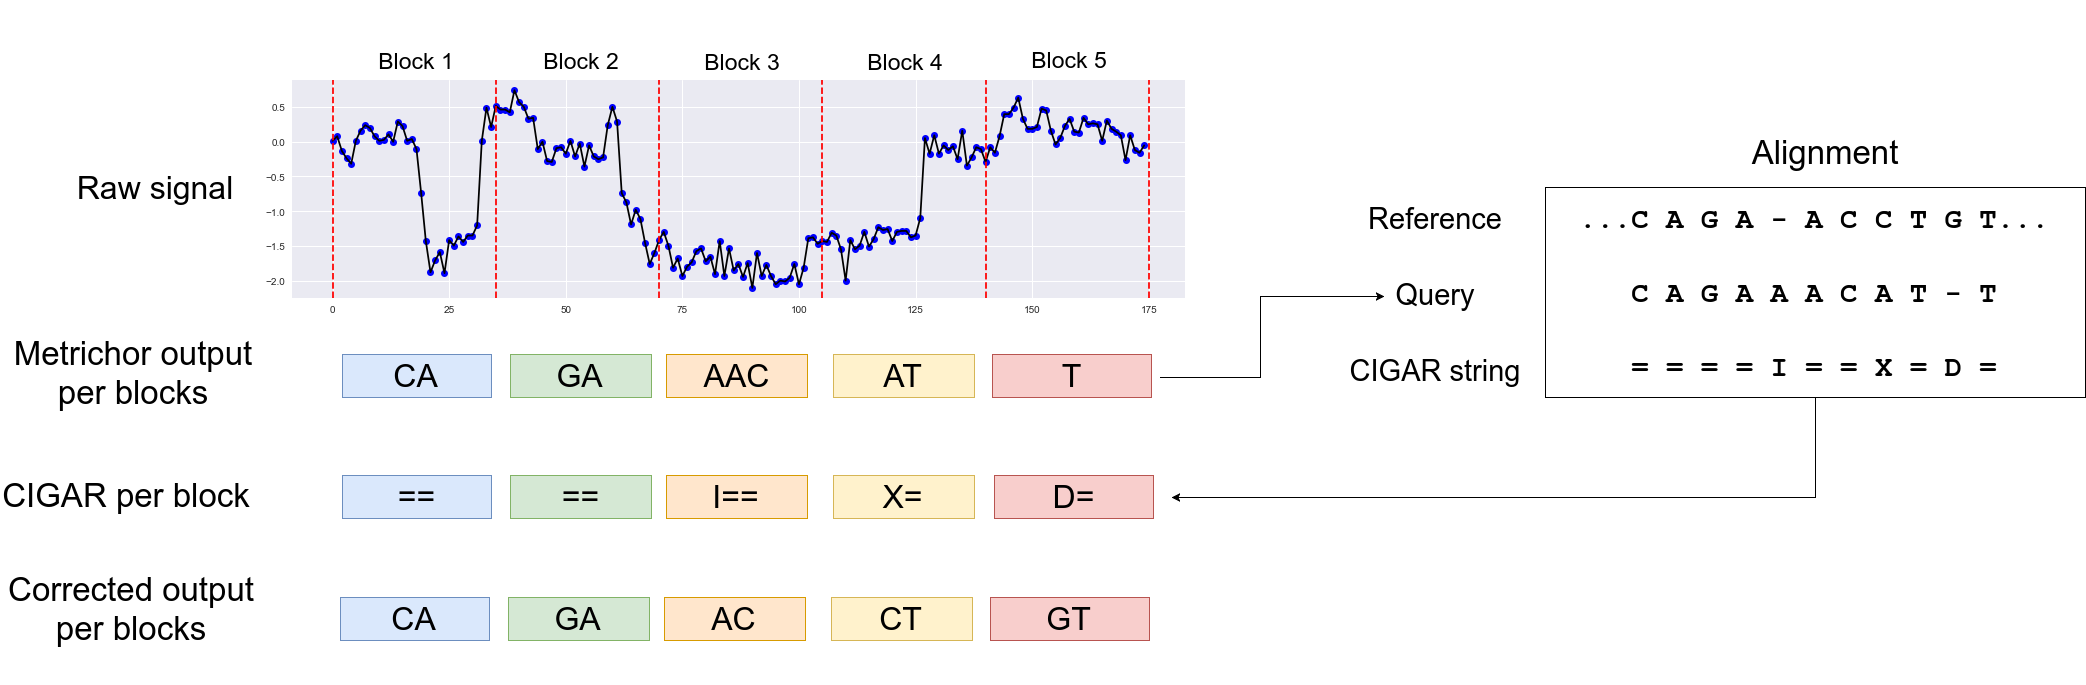
\includegraphics[width=1\textwidth]{./imgs/train_data_correction.png}
		\caption{Dataset preparation}
		\label{fg:data_correction}
	\end{center}
\end{figure}


To eliminate the possibility of overfitting to the known reference, the model is trained and tested on reads from different organisms. Due to limited amount of public available raw nanopore sequence data, ecoli was \textit{divided} into two regions.
Reads were split into train and test portions, depending on which region of ecoli they align. 
If read aligns inside first 70\% of the ecoli, it is placed into train set, and if it aligns to the second portion, it is placed into test set. Reads whose alignment overlaps train and test region are not used. Important to note that ecoli genome, and genomes of the majority of other bacteria, is cyclical, so reads with alignments that wrap over edges are also discarded. Total train set consist of over 110 thousand reads.
Overview of the entire learning pipeline is shown in figure \ref{fg:train_pipe}.
\begin{figure}[!ht]
	\begin{center}
		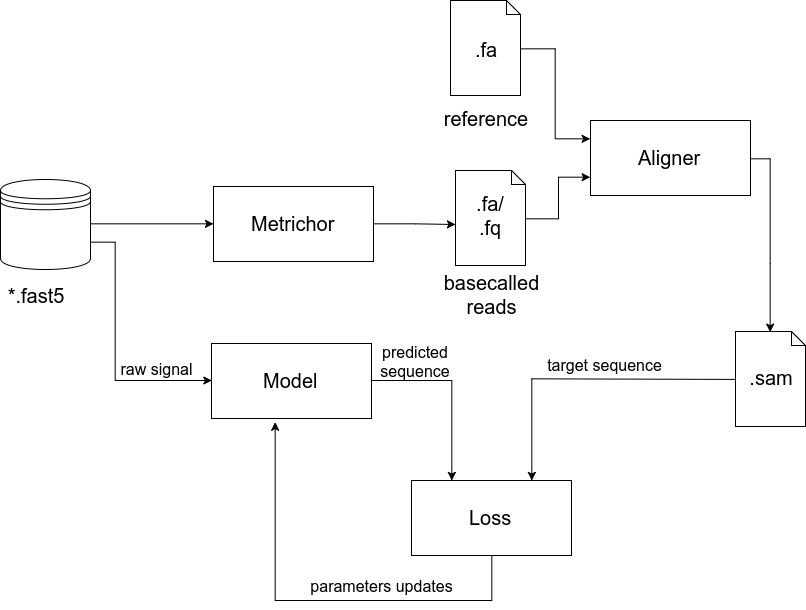
\includegraphics[width=0.7\textwidth]{./imgs/train_pipeline.png}
		\caption{Overview of training pipeline}
		\label{fg:train_pipe}
	\end{center}
\end{figure}

\section{Deep Learning model}

The final model is a residual neural network consisting of 72 residual blocks that are depicted in figure \ref{fg:model_block}. The used model is a variant of architecture proposed in paper \cite{identitet} with the difference of ELU being used as activation instead of ReLU as it is reported \cite{resnet-elu} to speeds up the learning process and improve accuracy as the depth increase.
\begin{figure}[!ht]
	\begin{center}
		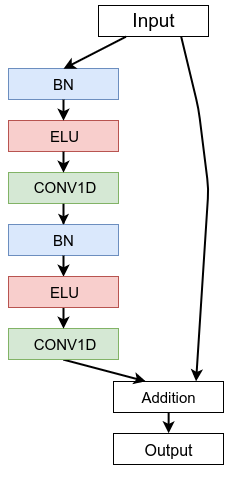
\includegraphics[width=0.2\textwidth]{./imgs/model.png}
		\caption{Used residual block}
		\label{fg:model_block}
	\end{center}
\end{figure} 

Each residual block contains two convolution layers making a total number of convolutions 144. Each convolutional layer in this models uses 64 kernels of 3. Because sequenced read is always shorter than the raw signal, pooling with kernel size two is used every 48 layers resulting in a reduction of dimensionality by factor 8. This is used reduce computation effort and to help training by reducing the number of required blank labels outputed by the network. This network has two million parameters that are learned during training. 

Training the model is the minimization of previously described CTC loss. It was done using Adam \cite{adam}, stochastic gradient descent algorithm based on an estimation of first and second-order moments.
It is often used as it offers fast and stable convergence. Default parameters of Adam were used (
$\beta_1=0.9$ and $\beta_2=0.999$). Initial learning rate was set to 1e-3 with exponential decay. Batch size was set to 8 mostly due to limited hardware resources. As noisy batches could potentially cause gradients to explode, gradient clipped to a range [-2, 2] was used.
Learning curve is show on figure \ref{fg:learn}. Occasional spikes of training loss are explained by small batch size and presence of noise in the signal. Learning curve shows no sign of overfitting as modes shows similar performance on both train and validation sets.

\begin{figure}[!ht]
	\begin{center}
		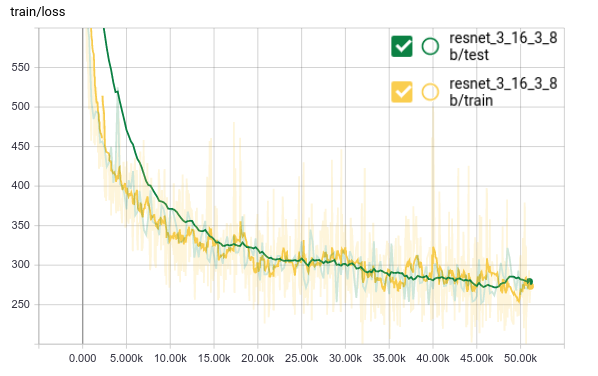
\includegraphics[width=0.6\textwidth]{./imgs/train_tb.png}
		\caption{Learning curve in TensorBoard}
		\label{fg:learn}
	\end{center}
\end{figure}

Training process is implemented as \textit{producers/consumer} pattern with communication done using FIFO\footnote{FIFO is an acronym for first in, first out} queue. Multiple producer threads, running on the CPU, load FAST5 and alimnment batch data, preprocess it and convert to required objects, while single GPU worker takes batch from the queue and computes forwards and backward passes on the network. This is done to reduce time between batches and maximize GPU utilization during training. 


\section{Technologies}
\label{sec:tech}
Overall solution was implemented in Python programing language. Described model is implemented using TensorFlow. It is an open source software library for numerical computation using data flow graphs developed by Google. TensorFlow, even though is considered low-level framework, offers implementations of many higher level concepts (layers, losses, and optimizers) which makes it great for prototyping while keeping it modular and extensible for highly specific tasks as well.

TensorFlow offers efficient GPU implementations of various layers and losses but as of version 1.2 still lacks GPU implementation of used CTC loss, so WARP-CTC\footnote{\url{https://github.com/baidu-research/warp-ctc}} was used. It offers both GPU and CPU implementations as well as bindings for TensorFlow.

For alignment tasks, developed tool offers support for GraphMap and BWA but can easily be extended with support any other aligner that outputs results in SAM file format.

SAMTools\footnote{\url{http://www.htslib.org/}} and Python bindings PySam\footnote{\url{https://github.com/pysam-developers/pysam}} were used for conversions between various file formats used in Bioinformatics.

Docker was used for automating the deployment on different machines. It helps to resolve problem know as \textit{dependency hell}\footnote{\url{https://en.wikipedia.org/wiki/Dependency_hell}}  keeping all dependencies in single container thus eliminating possible conflict between packages on host OS.
Nvidia Docker\footnote{\url{https://github.com/NVIDIA/nvidia-docker}} was used for GPU support inside docker containers.


Training and all evaluations were done on the server with  \textit{Intel(R) Xeon(R) E5-2640 CPU}, 600 GB of RAM and \textit{NVIDIA TITAN X Black} with 6GB of GDDR5 memory and 2880 CUDA cores.

All developed and used code, including utility scripts is publicly available on \textit{GitHub}\footnote{\url{https://github.com/mratkovic/masters-thesis}} under the \textit{MIT Licence}.

%%%%%%%%%%%%%%%%%%%%%%%%%%%%%%%%%%%%%%%%%%%%%%%%%%%%%%%%%%%%%%%%%%%%%%%%%%%%%%%%%%%%%%%
%% CHAPTER
\chapter{Results}
Developed tool was compared with other available basecallers that support R9 chemistry. This includes third-party basically DeepNano and official basecallers by Oxford Nanopore (cloud-based Metrichor and Nanonet).
The fact that ground truth is not known makes evaluation difficult. 
Different methods for evaluation were used to get clearer information about each basecaller.
In all tables and figures, developed model is addressed as \textit{resdeep} simply due to the fact it is a deep residual neural network.



\section{Error rates per read}

Basecalled reads are aligned to the reference using GraphMap and alignments are analyzed. If the whole sequencing is done correctly and quality basecaller is used, all reads should align to the reference. Mismatches, insertions, and deletions, in that case, should be due to limitations of sequencing technology and noise in the signal.

A portion of the read length that aligns as correctly is called match\_rate. Same goes for mismatches and insertions. 
Sum of all matches, mismatches, and insertions is equal to the reads length \ref{eq:read_len}. 

\begin{equation}
\begin{gathered}
\label{eq:read_len}
read\_len =  n\_matches + n\_mismatches + n\_insertions 
\end{gathered}
\end{equation}
\begin{equation}
\begin{gathered}
match\_rate = \dfrac{n\_matches}{read\_length}
\end{gathered}
\end{equation}
\begin{equation}
\begin{gathered}
missmatch\_rate = \dfrac{n\_mismatches}{read\_length}
\end{gathered}
\end{equation}
\begin{equation}
\begin{gathered}
insertion\_rate = \dfrac{n\_insertions}{read\_length}
\end{gathered}
\end{equation}

\begin{equation}
\begin{gathered}
match\_rate  + snp\_rate + insertion\_rate = 1
\end{gathered}
\end{equation}

Deletion rate is defined as a total number of deletions in the alignment over the length of the aligned read. 

\begin{equation}
\begin{gathered}
deletion\_rate = \dfrac{n\_deletion}{read\_length}
\end{gathered}
\end{equation}


To get reliable results, this is done on both ecoli test dataset and lambda dataset. 
For each basecaller, median, mean and variance of all aligned reads are calculated. To summarize the results, the median is used as a single value as it is robust and even more informative in the case of skewed distributions like these.  Results expressed as percentages are shown in the table \ref{tbl:ecoli_rates} for ecoli and table \ref{tbl:lambda_rates} for lambda dataset. 

Developed tool shows promising results by having better match rate and smaller mismatch rate than the others. 
Both datasets show all basecallers being biased towards deletions than insertions but this possibly is the bias of the used aligner. To eliminate that possibility, tests were repeated using \textit{BWA mem} aligner\footnote{https://github.com/lh3/bwa} with almost identical results. Results using BWA aligner are shown in tables
\ref{tbl:ecoli_rates_bwa} and \ref{tbl:lambda_rates_bwa}. Results are consistent on both datasets using both aligners.



\begin{table}[htb]
	\caption{Alignment specifications of Ecoli R9 basecalled reads using GraphMap}
	\label{tbl:ecoli_rates}
	\centering
	\begin{tabular}{lcccc}
		\toprule
		{} &  \thead{Match \% \\(median)} &  \thead{Mismatch \% \\(median)} &  \thead{Insertion \% \\(median)} &  \thead{Deletion \% \\(median)} \\
		\midrule
		
		DeepNano   &                  90.254762 &                      6.452852 &                       \textbf{3.274420} &                     11.829965 \\
		Metrichor  &                  90.560455 &                      5.688105 &                       3.660381 &                      8.328271 \\
		Nanonet    &                  90.607674 &                      5.608912 &                       3.652791 &                      8.299046 \\
		resdeep    &                  \textbf{91.408591} &                     \textbf{ 5.019141} &                       3.477739 &                      \textbf{7.471608 }\\
		\bottomrule
	\end{tabular}
\end{table}

\begin{table}[htb]
	\caption{Alignment specifications of Ecoli R9 basecalled reads using BWA mem}
	\label{tbl:ecoli_rates_bwa}
	\centering
	\begin{tabular}{lcccc}
		\toprule
		{} &  \thead{Match \% \\(median)} &  \thead{Mismatch \% \\(median)} &  \thead{Insertion \% \\(median)} &  \thead{Deletion \% \\(median)} \\
		\midrule
		DeepNano   &                  90.254762 &                      6.452852 &                       3.274420 &                     11.829965 \\
		Metrichor  &                  90.595441 &                      6.869543 &                       2.531646 &                      7.567381 \\
		Nanonet    &                  90.988989 &                      6.674760 &                     \textbf{  2.348552} &                      7.698530 \\
		resdeep    &                 \textbf{ 91.470588} &                      \textbf{5.929204 }&                       2.477283 &                     \textbf{ 6.970362} \\
		\bottomrule
	\end{tabular}
	
\end{table}
\begin{table}[htb]
	\caption{Alignment specifications of Ecoli R9 basecalled reads using GraphMap}
	\label{tbl:lambda_rates}
	\centering
	\begin{tabular}{lcccc}
		\toprule
		{} &  \thead{Match \% \\(median)} &  \thead{Mismatch \% \\(median)} &  \thead{Insertion \% \\(median)} &  \thead{Deletion \% \\(median)} \\
		\midrule
		DeepNano   &                  86.997687 &                      9.623494 &                       3.442490 &                     16.052830 \\
		Metrichor  &                  87.714988 &                      7.835052 &                       4.093851 &                     \textbf{10.757491} \\
		Nanonet    &                  88.415611 &                      8.178372 &                       3.629653 &                     11.793022 \\
		resdeep    &                 \textbf{ 89.694482} &                     \textbf{ 7.238095} &                       \textbf{3.078796} &                     13.450292 \\
		\bottomrule
	\end{tabular}
	
	
	
	
\end{table}
\begin{table}[H]
	\caption{Alignment specifications of lambda R9 basecalled reads using BWA mem}
	\label{tbl:lambda_rates_bwa}
	\centering
	\begin{tabular}{lcccc}
		\toprule
		{} &  \thead{Match \% \\(median)} &  \thead{Mismatch \% \\(median)} &  \thead{Insertion \% \\(median)} &  \thead{Deletion \% \\(median)} \\
		\midrule
		
		DeepNano   &                  86.625973 &                     11.288361 &                       2.098225 &                     14.648308 \\
		Metrichor  &                  87.294093 &                     10.109186 &                       2.376476 &                      \textbf{9.645323 }\\
		Nanonet    &                  87.767037 &                     10.017598 &                       2.354248 &                     10.597232 \\
		resdeep    &                 \textbf{ 89.049870} &                     \textbf{ 9.480883} &                       \textbf{1.615188 }&                     12.962441 \\
		\bottomrule
	\end{tabular}
	
\end{table}


Distribution of these percentages per reads are shown using  histogram plot on figure \ref{fg:hist} and the KDE (\textit{kernel density estimate}) plot on igures \ref{fg:ecoli_kde} and \ref{fg:lambda_kde}. Like the histogram, the KDE plot encodes the density of observations, but curve approximation is used instead of bins resulting in less cluttered comparison. 
It is important to note that lambda is small dataset and more samples are needed to get a better approximation of distribution.

\begin{figure}[!htb]
	\begin{center}
		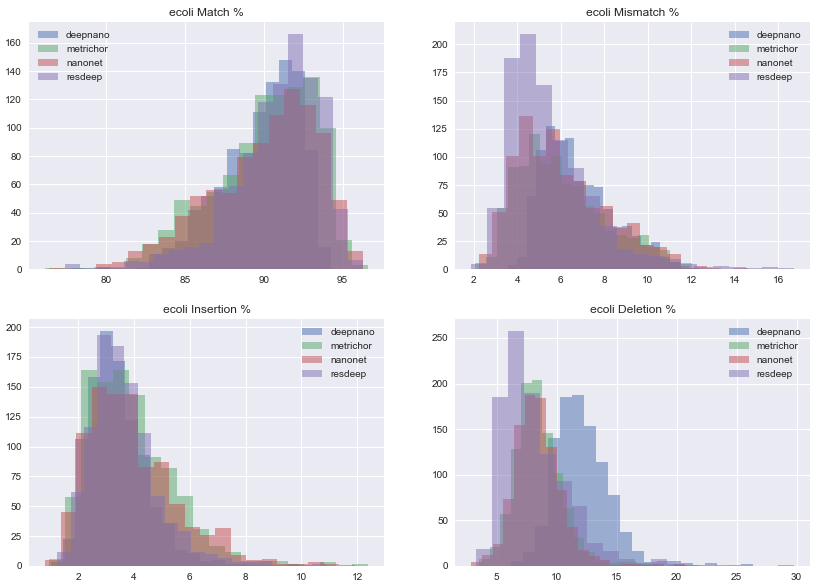
\includegraphics[width=0.8\textwidth]{./imgs/results/ecoli/hist_20.png}
		\caption{Histogram showing distribution of percentage of alimnment operations for ecoli}
		\label{fg:hist}
	\end{center}
\end{figure}

\begin{figure}[!htb]
	\begin{center}
		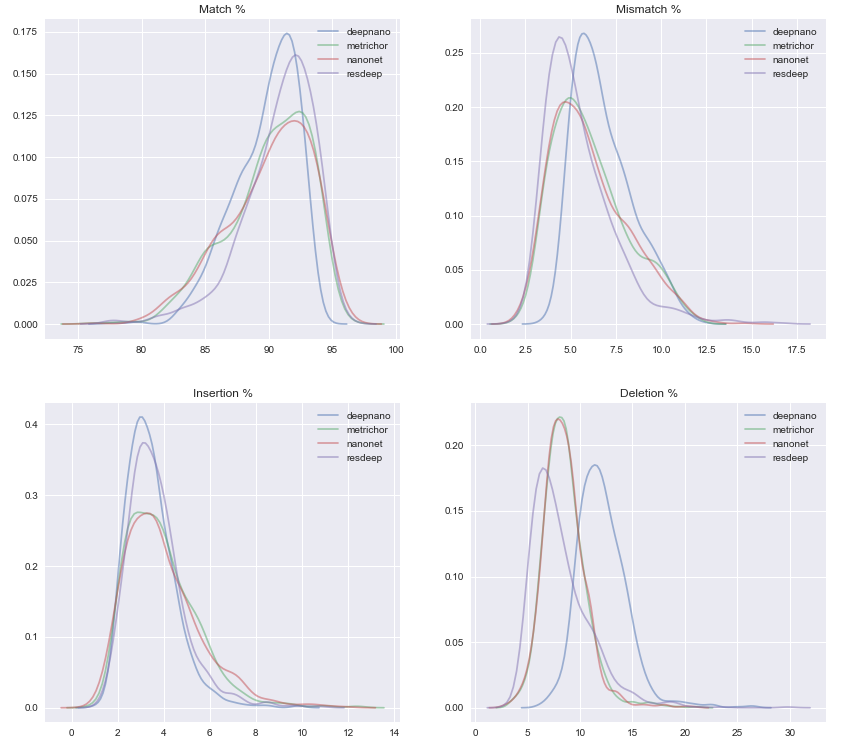
\includegraphics[width=0.8\textwidth]{./imgs/results/ecoli/kde_cigar.png}
		\caption{KDE plot for distribution of percentage of alimnment operations for ecoli}
		\label{fg:ecoli_kde}
	\end{center}
\end{figure}

\begin{figure}[!htb]
	\begin{center}
		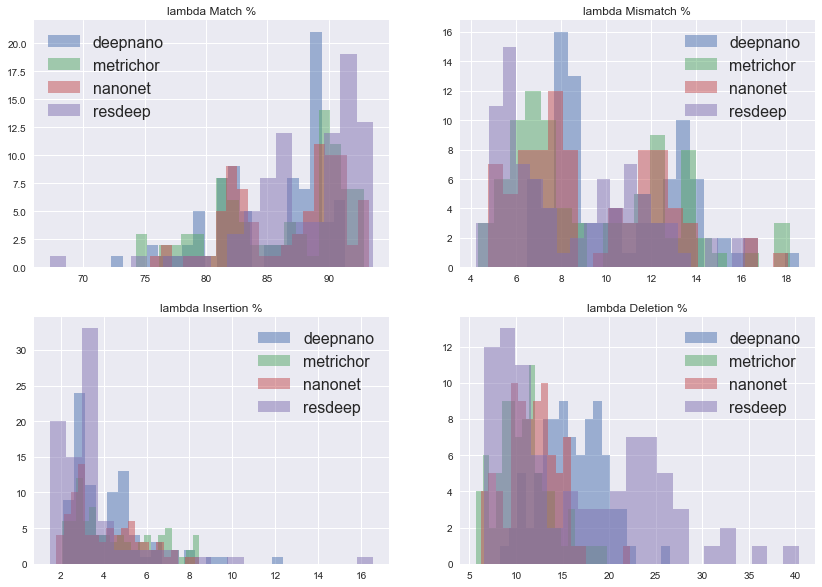
\includegraphics[width=0.8\textwidth]{./imgs/results/lambda/hist_20.png}
		\caption{Histogram showing distribution of percentage of alimnment operations for lambda}
		\label{fg:hist}
	\end{center}
\end{figure}

\begin{figure}[!htb]
	\begin{center}
		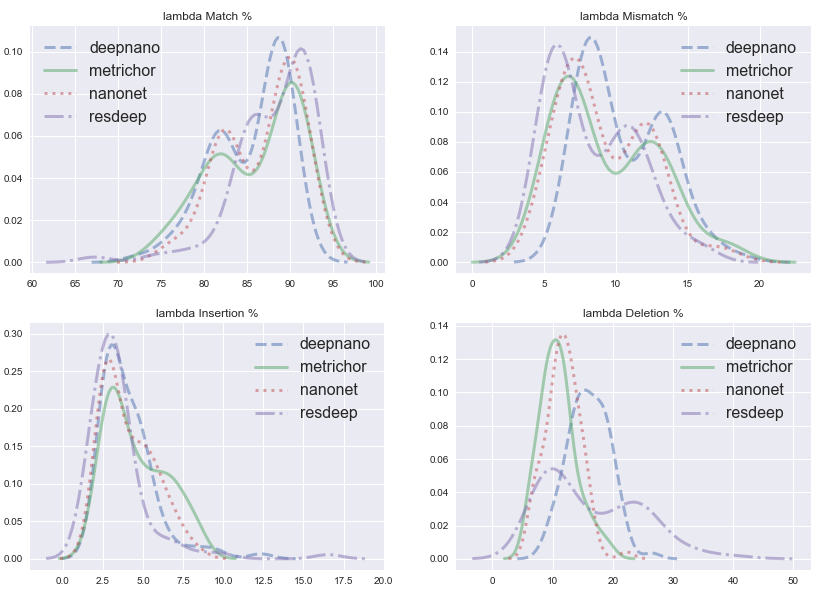
\includegraphics[width=0.8\textwidth]{./imgs/results/lambda/kde_cigar_lines.png}
		\caption{KDE plot for distribution of percentage of alimnment operations for lambda}
		\label{fg:lambda_kde}
	\end{center}
\end{figure}
\FloatBarrier

The histogram on figure \ref{fg:cigar_op_dist} shows how matches, mismatches, insertions, and deletions are distributed across the read. It is shown that mismatches and insertion occur more frequently at the beginnings and the ends of the reads. This is not only the case for the developed basecaller, but all other show the same property. This could be due to lack of context information from both sides when edges are base called.

\begin{figure}[!ht]
	\begin{center}
		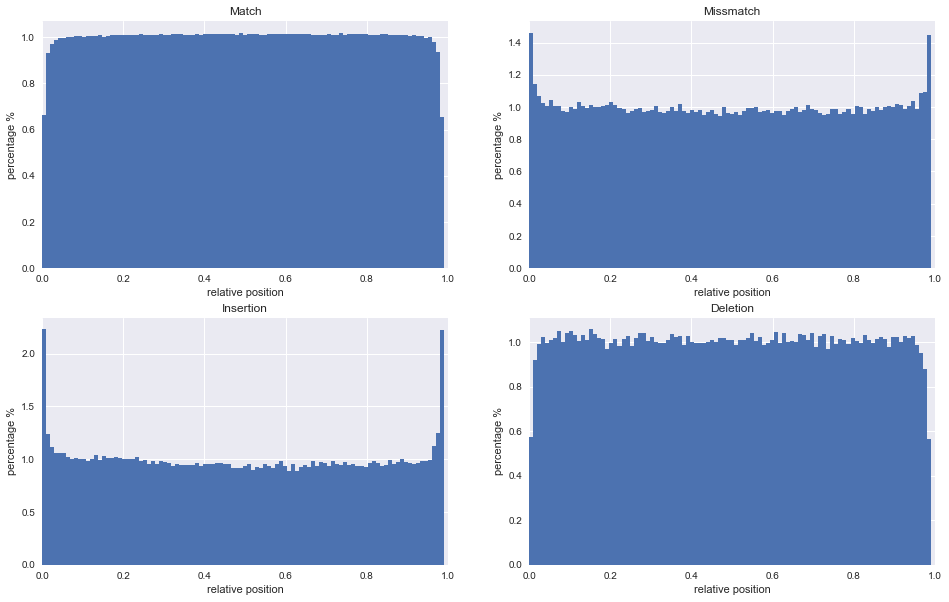
\includegraphics[width=1\textwidth]{./imgs/operation_distributed_r9.png}
		\caption{Histogram of alignment operations over relative position inside of read}
		\label{fg:cigar_op_dist}
	\end{center}
\end{figure}





\section{Consensus}
Described error rates and match rates calculated from alignments of individual reads to the reference could be misleading as it is simple to produce a naive model that obtains excellent results. Let us consider a model that basecalls single base "A" for every input signal. Aligning "A" to the reference (supposing that the aligner does not discard short and highly ambiguous reads) will always return perfect alignment as nucleotide "A" is certainly present in the reference. This model would have a perfect match rate with non-existent mismatches, insertions, and deletions. Two other approaches are used, in addition to the first, to give a more rigorous comparison.

The idea behind other approaches is checking if the reconstruction of the reference is possible from the basecalled reads and closely does it match the original reference.

\subsection{Consensus from pileup}
 Instead of going through the whole assembly process, as we know the reference genome of the data used in these tests, we simply align all the reads to the genome, stack them on top of each other forming pileup of read bases. Using majority vote, dominant bases are called on each position. The resulting sequence is called consensus. When calling consensus for deletions,  there has to be a majority of deletions of the same length. Calling insertions has the additional condition,  the majority has to agree on both length and the bases of insertion. Figure \ref{fg:consensus} shows how consensus is called from pileup created from aligned reads. Pileup is stored in mpileup format.  


\begin{figure}[!ht]
	\begin{center}
		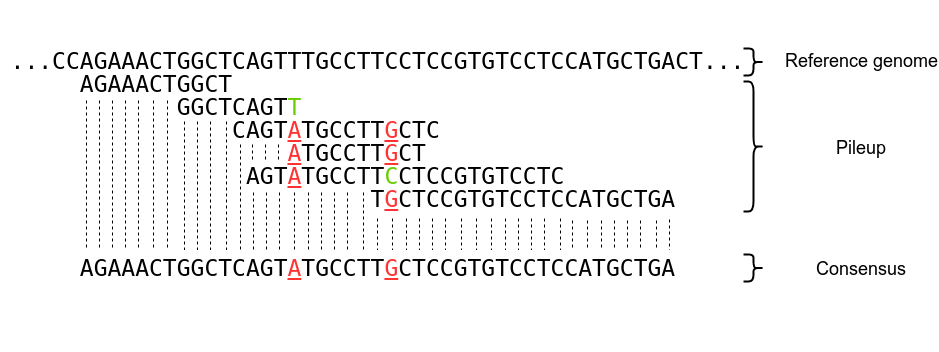
\includegraphics[width=0.8\textwidth]{./imgs/consnesus.png}
		\caption{Consensus from pileup}
		\label{fg:consensus}
	\end{center}
\end{figure}


Similarly, as before, match rate, mismatch rate, insertion and deletion rates are calculated but this time for whole consensus sequence. In this context, mismatches are called \textit{single nucleotide polymorphisms} (snp).



\begin{equation}
\begin{gathered}
match\_rate = \dfrac{n\_correct\_bases}{consensus\_length}
\end{gathered}
\end{equation}
\begin{equation}
\begin{gathered}
snp\_rate = \dfrac{n\_snp}{consensus\_length}
\end{gathered}
\end{equation}
\begin{equation}
\begin{gathered}
insertion\_rate = \dfrac{n\_insertions}{consensus\_length}
\end{gathered}
\end{equation}

\begin{equation}
\begin{gathered}
match\_rate  + snp\_rate + insertion\_rate = 1
\end{gathered}
\end{equation}


\begin{equation}
\begin{gathered}
deletion\_rate = \dfrac{n\_deletion}{consensus\_length}
\end{gathered}
\end{equation}

Results are shown in the tables \ref{tbl:spec_ecoli}  for ecoli and \ref{tbl:spec_lambda} for lambda. 
Developed model shows results comparable with Metrichor in all aspects (matches, mismatches, insertions, deletions and the total length of the consensus sequence) for lambda and show even better results from ecoli. 

\begin{table}[htb]
	\caption{Consensus specifications of Ecoli R9 basecalled reads}
	\label{tbl:spec_ecoli}
	\centering
	
	\begin{tabular}{lcccccc}
		\toprule
		{} &  \thead{Total called\\\lbrack bp\rbrack} &  \thead{Correctly called\\\lbrack bp\rbrack} &  \thead{Match\\\%} &  \thead{Snp\\\%} &  \thead{Insertion\\\%} &  \thead{Deletion\\\%} \\
		\midrule
		DeepNano  &                  1510244.0 &                      1493242.0 &          98.8742 &         1.0044 &               0.1214 &              0.9041 \\
		Metrichor &                  1515893.0 &                      1502588.0 &          99.1223 &         0.7464 &               0.1313 &              0.6300 \\
		Nanonet   &                  1414237.0 &                      1385515.0 &          97.9691 &         1.5700 &               0.4609 &              1.5158 \\
		resdeep   &                  1517828.0 &                      1506233.0 &          \textbf{99.2361} &         \textbf{0.6474} &               \textbf{0.1165} &             \textbf{ 0.5510 }\\
		\bottomrule
	\end{tabular}
	
\end{table}

\begin{table}[htb]
	\caption{Consensus specifications of lambda R9 basecalled reads}
	\label{tbl:spec_lambda}
	\centering
	
	\begin{tabular}{lcccccc}
		\toprule
		{} &  \thead{Total called\\\lbrack bp\rbrack} &  \thead{Correctly called\\\lbrack bp\rbrack} &  \thead{Match\\\%} &  \thead{Snp\\\%} &  \thead{Insertion\\\%} &  \thead{Deletion\\\%} \\
		\midrule
		DeepNano  &                    48342.0 &                        48025.0 &          99.3443 &         0.6433 &               \textbf{0.0124} &              0.2648 \\
		Metrichor &                    48469.0 &                        48257.0 &          \textbf{99.5626} &         \textbf{0.4188} &               0.0186 &              \textbf{0.1465} \\
		Nanonet   &                    48438.0 &                        48168.0 &          99.4426 &         0.5409 &               0.0165 &              0.1961 \\
		resdeep   &                    48385.0 &                        48163.0 &          99.5412 &         0.4402 &               0.0186 &              0.1976 \\
		\bottomrule
	\end{tabular}
\end{table}

All models show a slight bias towards deletions than insertions, but this may be the limitation of technology as it has been reported that deletion and mismatch rates for nanopore data are ordinarily higher than insertion rates \cite{sovic}.

\subsection{Assembly}
In this evaluation method, consensus sequence is not calculated from pileup, but by \textit{de novo} genome assembly. For this task, fast and accurate \textit{de novo} genome assembler \textit{ra}\footnote{\url{https://github.com/rvaser/ra}} \cite{vaser} was used and obtained consensus sequence is compared to the reference using \textit{dnadiff} present in the \textit{Mumer}\footnote{\url{https://github.com/garviz/MUMmer}}. 
The length of the reference, consensus sequence, number of contigs and percentages of aligned bases from the reference to the query and vice versa are shown in the table \ref{tbl:assembly}. Average identity summarizes how closely does the assembled sequence match the reference. This is run on full ecoli sequence run for 1D template reads (\textasciitilde 160k reads), for both developed tools, Nanonet and Metrichor. Developed tool has shown a small increase in quality of the assembled sequence over Metrichor by offering longer consensus, higher identity percentage, and overall smaller edit distance\footnote{Calculated using \url{https://github.com/isovic/racon/blob/master/scripts/edcontigs.py}}.


\begin{table}[htb]
	\caption{Assembly and consensus results for ecoli}
	\label{tbl:assembly}
	\centering

\begin{tabular}{lccc}
\toprule
&         Metrichor &           resdeep &          Nanonet \\
\midrule
\thead{Ref. genome size (bp)} &           4639675 &           4639675 &            4639675 \\
\thead{Total bases (bp)}      &           4604806 &           \textbf{4614354} &          4600056 \\
\thead{Contigs [\#]}           &                 1 &                 1 &                1 \\
\thead{Aln. bases ref. (bp)}  &  4639641(100.00\%) &  4639612(100.00\%) &  4639031(99.99\%) \\
\thead{Aln. bases query (bp)} &  4604787(100.00\%) &  4614351(100.00\%) &  4599745(99.99\%) \\
\thead{Avg. Identity}         &             98.76 &             \textbf{99.06} &            98.47 \\
\thead{Edit distance}         &             60418 &             \textbf{46686 }&            74341 \\
\bottomrule
\end{tabular}
\end{table}


\section{Read lengths}
The lengths of basecalled reads for each tool are interesting to analyze. Developed tool output reads of lengths similar to Metrichor while other tools, such as Nanonet, for instance, basecall reads that are significantly shorter. Detailed analysis of read length distributions is shown using KDE plots on figure \ref{fg:r_lens} for both lambda and ecoli.


\begin{table}[htb]
	\caption{Ecoli R9 basecalled read lengths in base pairs}
	\label{tbl:ecoli_lens}
	\centering
	
	\begin{tabular}{lccc}
		\toprule
		{} &  \thead{median} &   \thead{mean} &    \thead{std} \\
		\midrule
		DeepNano   &        5526.5 &  8126.694000 &  7406.554786 \\
		Metrichor  &        5809.5 &  8933.275000 &  9189.709720 \\
		Nanonet    &        3286.5 &  4874.406582 &  4803.182344 \\
		resdeep    &        5784.0 &  8990.988989 &  9297.972688 \\
		\bottomrule
	\end{tabular}
\end{table}


\begin{table}[htb]
	\caption{Lambda R9 basecalled read lengths in base pairs}
	\label{tbl:ecoli_lens}
	\centering
	
	\begin{tabular}{lccc}
		\toprule
		{} &  \thead{median} &    \thead{mean} &    \thead{std} \\
		\midrule
		DeepNano   &        4740.0 &   4664.750000 &  2628.512543 \\
		Metrichor  &        5491.0 &   5482.952941 &  2748.446253 \\
		Nanonet    &        4931.5 &   4925.804878 &  2739.987512 \\
		resdeep    &        5229.0 &   5138.764706 &  2605.958080 \\
		\bottomrule
	\end{tabular}
\end{table}

\begin{figure}[!ht]
	\begin{center}
		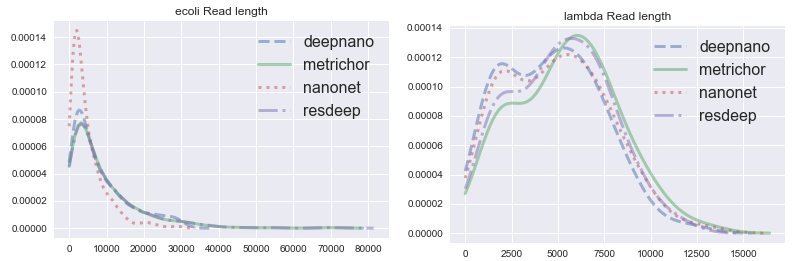
\includegraphics[width=1\textwidth]{./imgs/lens_lines.png}
		\caption{Overview of evaluation pipeline}
		\label{fg:r_lens}
	\end{center}
\end{figure}

\section{Base calling speeds}
Table \ref{tbl:speeds} shows base calling speeds of all tools. Metrichor is present in the table as it is cloud-based service and real execution time is unknown. Tests for all other basecallers were run under same conditions on hardware described in section \ref{sec:tech}. All tested tools offer parallelized base calling so a number of jobs(threads) during testing was set to 32. Both the developed model and Nanonet provide GPU support for base calling, while DeepNano is limited for CPU only.

Developed tool has shown faster base calling times in both CPU and GPU group even though it is very deep network of 144 layers. This shows efficiency of CNNs compared with RNNs. Differences in base calling speeds for ecoli and lambda datasets do exist, but they are not substantial and may be contributed to the different length of the reads and the different total number of reads in datasets. 

\begin{table}[htb]
	\caption{Base calling speeds measured in \textit{base pairs per second}}
	\label{tbl:speeds}
	\centering
	
	\begin{tabular}{lcc}
		\toprule
		{} &  \thead{ecoli (bp/s)} &  \thead{lambda (bp/s)} \\ 
		\midrule
		resdeep (CPU)  &               \textbf{1174.28} &              \textbf{ 1363.340 }\\
		Nanonet (CPU)  &                856.01 &                897.499 \\
		DeepNano (CPU) &                626.99 &                692.370 \\
		\midrule
		resdeep (GPU)  &              \textbf{ 6571.76 }&              \textbf{ 6140.300} \\
		Nanonet (GPU)  &               3828.39 &               3787.510 \\
		\bottomrule
	\end{tabular}
	
\end{table}

\section{Evaluation pipeline}
Entire evaluation pipeline is shown in figure \ref{fg:eval_pipe}.  GraphMap was used for alignment purposes and SAMTools for conversion between SAM and its binary variant BAM as well as a generation of mpileup.

\begin{figure}[!ht]
	\begin{center}
		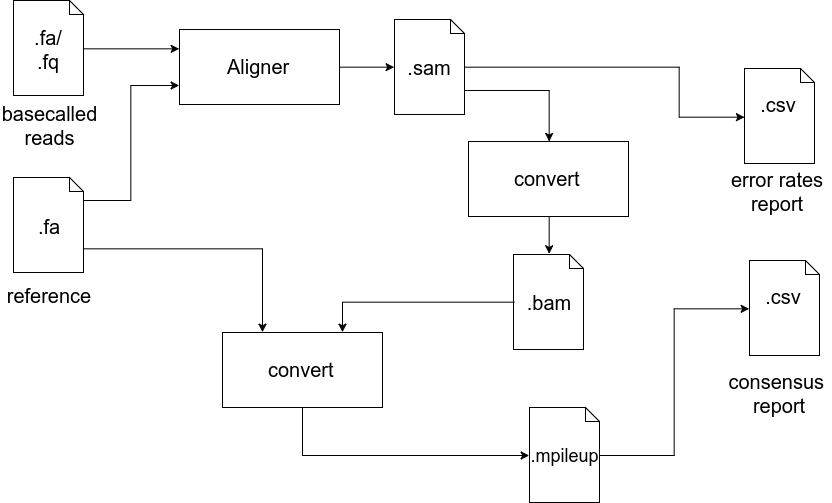
\includegraphics[width=0.7\textwidth]{./imgs/evaluation_pipeline.png}
		\caption{Overview of evaluation pipeline}
		\label{fg:eval_pipe}
	\end{center}
\end{figure}

%%%%%%%%%%%%%%%%%%%%%%%%%%%%%%%%%%%%%%%%%%%%%%%%%%%%%%%%%%%%%%%%%%%%%%%%%%%%%%%%%%%%%%%
%% CHAPTER
\chapter{Conclusion}



The goal of this thesis was to show that usage of convolution neural networks can potentially replace RNNs in the analysis of sequencing data by offering better results as well as faster execution times.

On all tests, proposed model has shown improvement in the accuracy of basecalled data as well as faster basecalling speeds of over both official (Matrichor and experimental Nanonet) and  third-party DeepNano while having. 
To provide definite proof of this claim, the model needs to be tested on larger datasets from different sequencing runs for multiple organisms.

All test are done on data for R9 chemistry, but the developed code could easily be adjusted and trained on R9.4 and newest R9.5 data when it becomes publicly available.
It would be interesting to see how well this approach works compare to basecaller Scrappie by Oxford Nanopore that addresses detection of homopolymers.

Currently, without support for newer sequencing data, this model has limited application. 
It can be used as a demonstration of a different approach to base calling which yields promising results.  As newer versions of basecallers by Oxford Nanopore do not offer any support for data sequenced with previous version of chemistries, this tool can be used to re-basecall that data and improvement of the quality of reads.

Future work includes experiments with recently proposed \textit{scaled exponential linear units} (SELU) \cite{selu} that eliminates the need for normalization techniques such as used batch normalization. Possible improvements of the model include the combination of convolutions and attention mechanism proposed just recently in the paper \cite{facebook} showing excellent results in both speed and accuracy, for tasks of language translation. 



%%%%%%%%%%%%%%%%%%%%%%%%%%%%%%%%%%%%%%%%%%%%%%%%%%%%%%%%%%%%%%%%%%%%%%%%%%%%%%%%%%%%%%%
%% DONE
\bibliography{references}
\bibliographystyle{unsrtnat}
\begin{abstract}


MinION by Oxford Nanopore Technologie is affordable and portable sequencing device suitable for various applications. The device produces very long reads, however, it suffers from high sequencing error rate. 
The goal of this thesis is to show that the reported accuracy of the sequencing data is not only limited by sequencing technology, but also by the current software tools used for base calling and can be further improved by using different deep learning concepts.
Approach for base calling of raw data using convolutional neural networks is proposed as an alternative to recurrent neural networks used by other basecallers offering improvements both in  speed and accuracy. A detailed comparison of the developed tool with the existing tools for base calling R9 data is given.

\keywords{base calling, Oxford Nanopore Technologies, MinION, deep learning, seq2seq, convolutional neural network, residual network, CTC loss}
\end{abstract}

\hrtitle{Model dubokog učenja za određivanje očitanih baza dobivenih uređajem za sekvenciranje MinION}
\begin{sazetak}


Uređaji za sekvenciranje MinION tvrtke Oxford Nanopore Technologies su pristupačni i prenosivi što ih čini pogodnim za razne primjene. 
Uređaj omogućuje sekvenciranje očitanja velikih duljina ali većeg postotka greške u odnosu na prethodne tehnologije.
Cilj ovog diplomskog rada je pokazati da trenutna pogreška nije uzrokovana isključivo metodom sekvenciranja, već i programskim alatima koji se koriste za očitavanje baza te je pogrešku moguće smanjiti korištenjem metoda dubokog učenja.

Predstavljen je novi alat za očitavanje baza temeljen na konvolucijskim neuronski mrežama koji pruža napredak u preciznosti i brzini u odnosu na trenutno korištene rekurzivne neuronske mrežama. U radu je dana detaljna analiza razvijenog alata i usporedba s postojećim rješenjima za određivanje očitanih baza.

\kljucnerijeci{određivanje baza, Oxford Nanopore Technologies, MinION, duboko učenje, prevođenje, konvolucijske neuronske mreže, rezidualne mreže, CTC gubitak}
\end{sazetak}

\end{document}
